\noindent\textbf{Thread}
\begin{itemize}
    \item single unique execution context: fully describes program state
    \item Program Counter, Registers, Execution Flags, Stack
\end{itemize}
\textbf{Address space (with translation)}
\begin{itemize}
    \item Programs execute in an address space that is distinct from the memory
space of the physical machine
\end{itemize}
\textbf{Process}
\begin{itemize}
    \item An instance of an executing program is a process consisting of an address space and one or more threads of control
\end{itemize}
\textbf{Dual mode operation / Protection}
\begin{itemize}
    \item Only the ``system'' has the ability to access certain resources
    \item The OS and the hardware are protected from user programs and user programs are isolated from one another by controlling the translation from program virtual addresses to machine physical addresses
\end{itemize}
\begin{discussion}
How do we run programs?
\end{discussion}
\begin{figure}[H]
    \centering
    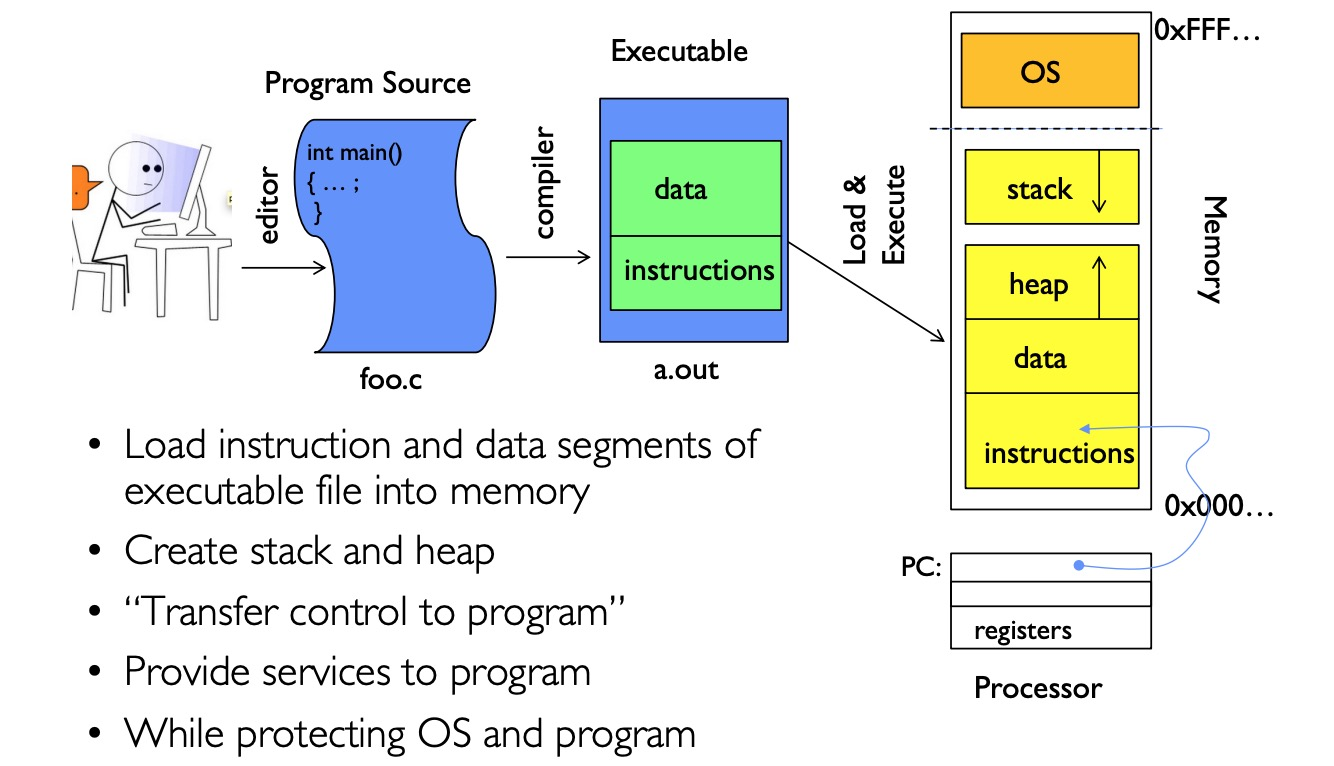
\includegraphics[width = 0.6\textwidth ]{figures/run_program.jpg}
    \caption{Run a Program}
    % \label{fig:batteryIncreas}
\end{figure}

\begin{discussion}
What happens during program execution?
\end{discussion}
\begin{figure}[H]
    \centering
    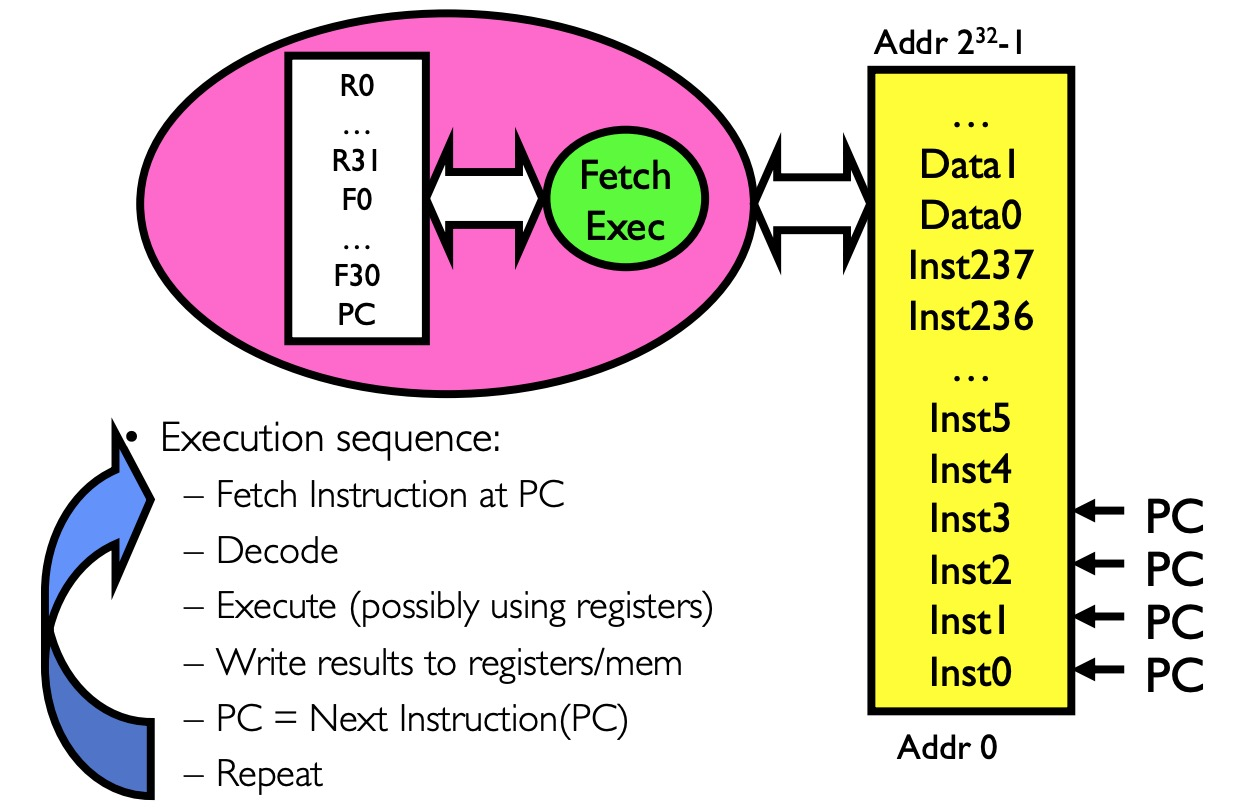
\includegraphics[width = 0.6\textwidth ]{figures/What_happens_during_program_execution?.jpg}
    \caption{What happens during program execution?}
    % \label{fig:batteryIncreas}
\end{figure}
\subsection{First OS Concept: Thread of Control}
\textbf{Thread}: Single unique execution context: \textbf{Program Counter, Registers, Execution Flags, Stack}
\begin{itemize}
    \item \textbf{Certain registers} hold the context of thread
    \item A thread is executing on a processor when it is resident in the processor register
    \item PC register holds the address of executing instruction in the thread
    \item Registers hold the root state of the thread
    \begin{itemize}
        \item The rest is ``in memory''
    \end{itemize}
\end{itemize}


\subsection{Second OS Concept: Program's Address Space}

\subsection{Third OS Concept: Process}
\begin{figure}[H]
    \centering
    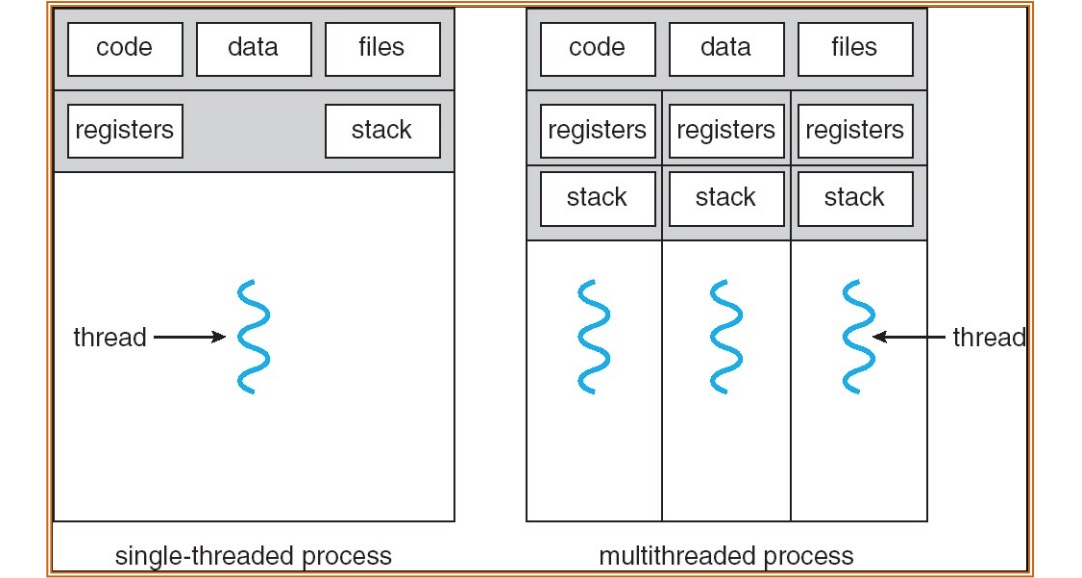
\includegraphics[width = 0.6\textwidth ]{figures/process.jpg}
    \caption{Single and Multithreaded Processes}
    % \label{fig:batteryIncreas}
\end{figure}


\subsection{Fourth OS Concept: Dual Mode Operation}
\begin{figure}[H]
    \centering
    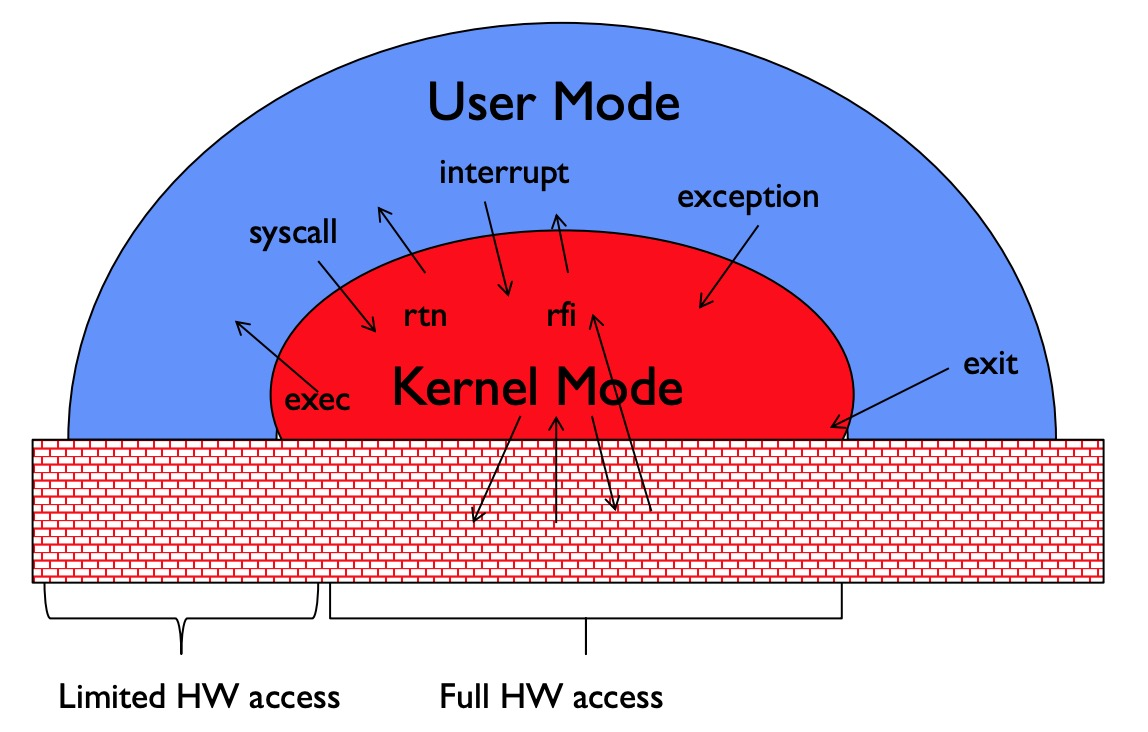
\includegraphics[width = 0.6\textwidth ]{figures/dual_mode.jpg}
    \caption{User/Kernel (Privileged) Mode}
    % \label{fig:batteryIncreas}
\end{figure}
\subsubsection{3 types of Mode Transfer}
\begin{itemize}
    \item \textbf{Syscall}
    \begin{itemize}
        \item Process requests a system service, e.g., exit
        \item Like a function call, but ``outside'' the process
        \item Does not have the address of the system function to call
        \item Like a Remote Procedure Call (RPC)
        \item Marshall the syscall id and args in registers and exec syscall
    \end{itemize}
    \item \textbf{Interrupt}
    \begin{itemize}
        \item External asynchronous event triggers context switch
        \item e. g., Timer, I/O device
        \item \textbf{Independent} of user process
    \end{itemize}
    \item \textbf{Trap or Exception}
    \begin{itemize}
        \item Internal synchronous event in process triggers context switch
        \item e.g., Protection violation (segmentation fault), Divide by zero, \dots
    \end{itemize}
\end{itemize}